\chapter{Introduction}
If there are two characteristics the internet has shown over the past 30 years, it's spacial growth, and an insatiable demand for bandwidth.
By December 2010, almost 30\% of the world's population was connected to the Internet. In the developing world, much of this can be accredited to the growth of mobile connectivity, but even for DSL, a technology that dates back to 1984, growth continues. In Q3 2010, BT announced that it had added nearly 200,000 DSL lines in the UK, bringing their total market share to 53\%.\cite{BP11}

The rise of applications including  live-video streaming such as BBC iPlayer, distributed content systems such as BitTorrent, and real-time gaming platforms such as XBox Live, continuously pressure Internet Service Providers (ISP\nomenclature{ISP}{Internet Service Provider}'s) to improve backbone and last-mile infrastructure to satisfy customer expectations.
Technologies are coming to market, such as Fibre to the Home/Building/Cabinet (FTTx\nomenclature{FTTx}{Fibre-to-the Home/Building/Cabinet}) which involves the replacement of copper lines with optical fibres, but in many cases, this is expensive and will not be done outside of dense municipal areas.

\begin{figure}[ht!]
 \centering
 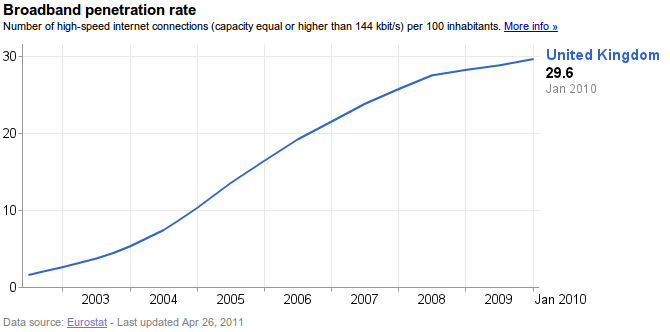
\includegraphics[width=0.45\textwidth]{images/BT-DSL-growth.png}
 \caption{Growth in Broadband connections in the UK}
 \label{fig:bt-dsl-stats}
\end{figure}

For other users, Digital Subscriber Lines (DSL) built on top of the existing plain old telephone system (POTS\nomenclature{POTS}{Plain Old Telephone Service}) are often the only option for anything approaching high-speed internet access. As such, DSL has been a focus of research and development, leading to significant growth in achievable data rates, from 8MBits Downstream for Asymmetric DSL (ADSL\nomenclature{ADSL}{Asymmetric Digital Subscriber Lines}) , through 24 MBits Downstream for ADSL2/2+, and more recently, up to 100MBits symmetrically on short loop lengths (less than 250m) for Very high bit-rate DSL (VDSL\nomenclature{VDSL}{Very high bit-rate Digital Subscriber Lines}).

FTTx and xDSL are both evolving together; as FTTx reduces the last-mile length, xDSL frequency use expands to provide the maximum bandwidth on that short-loop. While in some urban areas, FTTH will become the prevalent form of broadband internet access, xDSL will still be needed for a long time to come for the vast majority of the populace.

But existing methods of managing the bandwidth allocations for bundles of xDSL lines are either computationally simple, but sub-optimal, or computationally intractable and near-optimal. Much work and research has gone into developing advanced and intelligent Dynamic Spectrum Management (DSM) algorithms, but little attention has been applied to the practical implications of these algorithms and the real-world effect that different forms of that implementation make to performance and tractability.

Massively parallel computing, in the form of GPGPU, is becoming a popular paradigm in computational research, with classically linear algorithms being distributed across these Single Instruction Multiple Data (SIMD) devices giving general speed-ups in the range of 5-500x. The most popular and developed form of GPGPU architecture is NVidia's Compute Unified Device Architecture (CUDA\nomenclature{CUDA}{Compute Unified Device Architecture}), which leverages the streaming multiprocessor (SM\nomenclature{SM}{Streaming Multiprocessor}) and high speed memories of their GPU's (usually used for gaming) for use as scientific computation devices. 

In this report, the viability of GPGPU accelerated DSM algorithms is investigated, 
\clearpage
\section{Project Specification}
\label{sec:proj-spec}
\begin{centering}
\textbf{School of Electrical and Electronic Engineering and Computer Science\\
FINAL YEAR PROJECT 2010/2011\\}
\end{centering}

\begin{tabular}{rl}
\\\\Title:&High-Speed bit-loading algorithms for Dynamic Spectrum Management in ADSL\\
Student:&Andrew Bolster\\
Supervisor:&Prof A Marshall\\
Moderator:&Dr J McAllister\\
Area:&Digital Comms\\
Research Cluster:&Digital Comms\\\\
\end{tabular}

Digital subscriber lines need to employ bit-loading techniques to improve their throughput; this is known as “Dynamic Spectrum Management” (DSM). Currently all implementations of DSM use level 1 whereby individual lines use a “water-filling” algorithm to adjust the power allocated to each tone in the spectrum, and a central management station adjusts the water-filling parameters for each line in the subscriber bundle. However this approach is sub-optimal whenever the capacity of the overall bundle is considered, hence more recent research has proposed (level 2) more intelligent methods to allocate the power for each bit in each tone, considering both near and far end crosstalk in the bundle.
A major problem with the level 2 techniques is their computational complexity which currently renders them practically infeasible, e.g. ISB typically takes more than 1 week to compute the tones for a 10-line bundle. Graphic Processing Units (GPUs) represent a new approach to massively parallel floating-point computations. Moreover the Compute Unified Device Architecture (CUDA) developed by NVidia,represents a framework whereby new highly parallel algorithms can be developed. The main aim of this project is to apply this approach to level 2 DSM algorithms, many of which are highly parallel in their operation.

\textbf{The objectives of the project are:}
\begin{enumerate*}
 \item Become familiar with DSM techniques for Digital Subscriber Lines.
 \item Become familiar with the CUDA environment for GPU's and identify a suitable platform.
 \item Investigate efficient implementations of level 2 DSM.
 \item Develop an implementation of a level 2 bit-loading algorithm using GPU's.
\end{enumerate*}

\textbf{M.Eng. Extensions}
\begin{enumerate*}
 \item Analyse the performance of your implementation in terms of speed, cost, and scalability (number of lines).
 \item Compare your design with existing implementations.
\end{enumerate*}

\textbf{Learning Outcomes}
\begin{enumerate*}
 \item Understand how to use CUDA to programme GPU's.
 \item Be able to design bit-loading algorithms for DMT.
 \item How to analyse the performance of an implementation.
\end{enumerate*}

\section{Overview and Objectives}
\label{sec:overview}
The project specification is quite expansive, covering a vast range of areas that I have not encountered directly in my studies but have tangentially met externally. Parallel computation is an active area of research, especially Massively Parallel GPGPU systems such as this. Additionally, there are almost as many DSM algorithms as there are DSM researchers, so algorithm selection and implementation must be very carefully planned and executed to keep within a workable time-frame.

As with any project of this scale, the necessary first stage is a thorough investigation of the problem. Not only the areas of DSM directly relevant to the Level 2 algorithms under analysis, but also the underlying DSL technology to enable generation and implementation of a computational model on which to test the algorithms. This will necessitate the selection of a programming environment that must be held consistent throughout the project, as well as the additional implementation of Optimal Spectrum Balancing (OSB) for comparative analysis. In the interests of not reinventing the wheel, research will also be undertaken to assess the usefulness of any existing DSL models / DSM implementations in terms of development guidance.

Beyond the problem itself, technologies involved in the suggested solution will have to be expansively researched, such as CUDA, GPGPU, and Computational Parallelism, including any recent relevant scholarly works that could be useful.

To summarise, the main points that need investigation will be:

\begin{itemize*}
 \setlength{\itemsep}{0.75pt}
 \setlength{\parskip}{0pt}
 \setlength{\parsep}{0pt}

 \item Problem Research
  \begin{itemize*}
   \item How DSL works
   \item DMT communications
   \item Dynamic Spectrum Management
   \item DSM Levels
   \item Existing/previous DSL simulation systems
   \item Existing/previous DSM implementations
  \end{itemize*}
 \item Solution Research
  \begin{itemize*}
   \item Relevant Programming Environments
   \item Software Profiling
   \item Massively Parallel Computing
   \item Parallel Computing Architectures
   \item CUDA software considerations
   \item CUDA hardware considerations
  \end{itemize*}
 \item Development
  \begin{itemize*}
   \item Design and implement DSL system model simulator
   \item Implement Optimal Spectrum Balancing (OSB\nomenclature{OSB}{Optimal Spectrum Balancing}) algorithm
   \item Implement Greedy bit-loading algorithm (MIPB\nomenclature{MIPB}{Multi-user Incremental Power Balancing, aka Greedy}) algorithm
   \item Implement Iterative Spectrum Balancing (ISB\nomenclature{ISB}{Iterative Spectrum Balancing}) algorithm
   \item Evaluate system performance through the use of profilers and workload visualisation
   \item Develop single-device GPU versions of above algorithms
   \item Evaluate performance of these algorithms, with respect to CPU\nomenclature{CPU}{Central Processing Unit}-bound versions
   \item If viable, implement multi-GPU versions of above algorithms
  \end{itemize*}
 \item Analysis
   \begin{itemize*}
    \item Compare and contrast performance concerns and resource usage of differing implementations
    \item Evaluate system cost concerns, and potential future avenues of development.
   \end{itemize*}
\end{itemize*}
